%%% Exemplo de utilização da classe ITA
%%%
%%%   por        Fábio Fagundes Silveira   -  ffs [at] ita [dot] br
%%%              Benedito C. O. Maciel     -  bcmaciel [at] ita [dot] br
%%%              Giovani Volnei Meinertz   -  giovani [at] ita [dot] br
%%%    	         Hudson Alberto Bode       -  bode [at] ita [dot]br
%%%    	         P. I. Braga de Queiroz    -  pi [at] ita [dot] br
%%%    	         Jorge A. B. Gripp         -  gripp [at] ita [dot] br
%%%    	         Juliano Monte-Mor         -  jamontemor [at] yahoo [dot] com [dot] br
%%%    	         Tarcisio A. B. Gripp      -  tarcisio.gripp [at] gmail [dot] com
%%%    	         
%%%
%%%  IMPORTANTE: O texto contido neste exemplo nao significa absolutamente nada.  :-)
%%%              O intuito aqui eh demonstrar os comandos criados na classe e suas
%%%              respectivas utilizacoes.
%%%
%%%  Tese.tex  2015-04-08
%%%  $HeadURL: http://www.apgita.org.br/apgita/teses-e-latex.php $
%%%
%%% ITALUS
%%% Instituto Tecnológico de Aeronáutica --- ITA, Sao Jose dos Campos, Brasil
%%%                   http://groups.yahoo.com/group/italus/
%%% Discussion list: italus {at} yahoogroups.com
%%%
%++++++++++++++++++++++++++++++++++++++++++++++++++++++++++++++++++++++++++++++
% Parametros da classe ITA para inserir em \documentclass[?]{?}
%   tg       = Trabalho de Graduacao
%   tgfem    = Para Engenheiras
%   msc      = Dissertacao de Mestrado
%   mscfem   = Para Mestras
%   dsc      = Tese de Doutorado
%   dscfem   = Para Doutoras
%   quali    = Exame de Qualificacao
%   qualifem = Exame de Qualificacao para Doutoras
%   dv       = 'Draft Version'     --> imprime 'Versao Preliminar + data no rodape
%   eng      = para teses em inglês
%++++++++++++++++++++++++++++++++++++++++++++++++++++++++++++++++++++++++++++++
%se fosse em inglês: \documentclass[dsc, eng]{ita}
%para ``draft version'': \documentclass[dsc, dv]{ita} ou \documentclass[dsc, eng, dv]{ita}

\documentclass[tg]{ita}    % ITA.cls based on standard book.cls 
% Quando alterar a classe, por exemplo de [msc] para [msc, eng]) rode mais uma vez o botão BUILD OUTPUT caso haja erro
\usepackage{ae}
\usepackage{graphicx}
\usepackage{epsfig}
\usepackage{amsmath}
\usepackage{amssymb} 
\usepackage{subfig}
\usepackage{multirow}
\usepackage{float}
\usepackage[table,xcdraw]{xcolor}

%++++++++++++++++++++++++++++++++++++++++++++++++++++++++++++++++++++++++++++++
% Espaçamento padrão de todo o documento
%++++++++++++++++++++++++++++++++++++++++++++++++++++++++++++++++++++++++++++++
\onehalfspacing

%singlespacing Para um espaçamento simples
%onehalfspacing Para um espaçamento de 1,5
%doublespacing Para um espaçamento duplo

%++++++++++++++++++++++++++++++++++++++++++++++++++++++++++++++++++++++++++++++
% Identificacoes (se o trabalho for em inglês, insira os dados em inglês)
% Para entradas abreviadas de Professora (Profa.) em português escreva: Prof$^\textnormal{a}$.
%++++++++++++++++++++++++++++++++++++++++++++++++++++++++++++++++++++++++++++++
\course{Engenharia de Computação} % Programa de PG ou Curso de Graduação
\area{Sistemas Aeroespaciais e Mecatr\~{o}nica} % Área de concentração na PG (Não utilizado no caso de TG)
\dept{Engenharia de Computação} % Divisão Acadêmica no ITA

% Autor do trabalho: Nome Sobrenome
\authorgender{masc}                     %sexo: masc ou fem
\author{Lucas Muller Machado}{de Oliveira}
\itaauthoraddress{Rua H8A, 139}{12.228-460}{São José dos Campos--SP}

% Titulo da Tese/Dissertação
\title{Um Estudo de Entropia em Composições Musicais}

% Orientador
\advisorgender{masc}                    % masc ou fem
\advisor{Prof.~Dr.}{Manish Sharma}{ITA}

% Coorientador (Caso não haja coorientador, colocar ambas as variáveis \coadvisorgender e \coadvisor comentadas, com um % na frente)
% \coadvisorgender{fem}									% masc ou fem
% \coadvisor{Prof$^\textnormal{a}$.~Dr$^\textnormal{a}$.}{Doralice Serra}{OVNI}

% Pró-reitor da Pós-graduação
\bossgender{masc}												% masc ou fem
\boss{Prof.~Dr.}{John von Neumann}

%Coordenador do curso no caso de TG
\bosscoursegender{fem}									% masc ou fem
\bosscourse{Prof.~Dr.}{Cecília de Azevedo Castro César}

% Palavras-Chaves informadas pela Biblioteca -> utilizada na CIP
\kwcip{Entropia}
\kwcip{Música}
\kwcip{Teoria da Informação}

% membros da banca examinadora

\examiner{Prof. Dr.}{Manish Sharma}{}{ITA}
\examiner{Prof. Dr.}{Marcelo Pinho}{}{ITA}
\examiner{Prof. Dr.}{Nei Soma}{}{ITA}

% Data da defesa (mês em maiúsculo, se trabalho em inglês, e minúsculo se trabalho em português) 
\date{21}{novembro}{2017}

% Número CDU - (somente para TG)
\cdu{681.3:534.323} % número CDU para TG

% Glossario
\makeglossary
\frontmatter

\begin{document}
% Folha de Rosto e Capa para o caso do TG
\maketitle

% Dedicatoria: Nao esqueca essa secao  ... :-)
\begin{itadedication}
Aos meus pais, que muito fizeram para que eu chegasse até aqui.
\end{itadedication}

% Agradecimentos
\begin{itathanks}
Agradeço primeiramente a Deus, que esteve comigo em toda minha caminhada.

Agradeço aos meus pais, que sempre estiveram do meu lado me motivando e fazendo de tudo para que eu alcançasse o que eu alcancei, e também a toda minha família.

Agradeço a todos os professores que, ao longo dos anos, contribuiram com a minha formação.

Agradeço a meus amigos, antigos e novos, que sempre estiveram comigo compartilhando dos bons e maus momentos.


\end{itathanks}

% Epígrafe
\thispagestyle{empty}
\ifhyperref\pdfbookmark[0]{\nameepigraphe}{epigrafe}\fi
\begin{flushright}
\begin{spacing}{1}
\mbox{}\vfill
{\sffamily\itshape
``Woof, Woof!''\\}
--- \textsc{Routh Hurwitz  }
\end{spacing}
\end{flushright}

% Resumo
\begin{abstract}
TODO:

Aqui começa o resumo do referido trabalho. Não tenho a menor idéia do que colocar aqui. Sendo assim, vou inventar. Lá vai: Este trabalho apresenta uma metodologia de controle de posição das juntas passivas de um manipulador subatuado de uma maneira subótima. O termo subatuado se refere ao fato de que nem todas as juntas ou graus de liberdade do sistema são equipados com atuadores, o que ocorre na prática devido a falhas ou como resultado de projeto. As juntas passivas de manipuladores desse tipo são indiretamente controladas pelo movimento das juntas ativas usando as características de acoplamento da dinâmica de manipuladores. A utilização de redundância de atuação das juntas ativas permite a minimização de alguns critérios, como consumo de energia, por exemplo.
Apesar da estrutura cinemática de manipuladores subatuados ser idêntica a do totalmente atuado, em geral suas caraterísticas dinâmicas diferem devido a presença de juntas passivas. Assim, apresentamos a modelagem dinâmica de um manipulador subatuado e o conceito de índice de acoplamento. Este índice é utilizado na sequência de controle ótimo do \mbox{manipulador}.
A hipótese de que o número de juntas ativas seja maior que o número de
passivas  $(n_{a} > n_{p})$  permite o controle ótimo das juntas passivas, uma vez que na etapa
de controle destas há mais entradas (torques nos atuadores das juntas ativas), que
elementos a controlar (posição das juntas passivas). 
\end{abstract}

% Abstract
\begin{englishabstract}
TODO:

Well, the book is on the table. This work presents a control methodologie for the position of the  passive joints of an underactuated manipulator in a suboptimal way. The term underactuated refers to the fact that not all the joints or degrees of freedom of the system are equipped with actuators, which occurs in practice due to failures or as design result. The passive joints of manipulators like this are indirectly controlled by the motion of the active joints using the dynamic coupling characteristics. The utilization of actuation redundancy of the active joints allows the minimization of some criteria, like energy consumption, for example. Although the kinematic structure of an underactuated manipulator is identical to that of a similar fully actuated one, in general their dynamic characteristics are different due to the presence of passive joints. Thus, we present the dynamic modelling of an underactuated manipulator and the concept of coulpling index. This index is used in the sequence of the optimal control of the manipulator.

\end{englishabstract}

% Lista de figuras
\listoffigures %opcional

% Lista de tabelas
\listoftables %opcional

% Lista de abreviaturas
\listofabbreviations
\begin{longtable}{ll}
TODO:
MIDI & Musical Instrument Digital Interface

CTq & computed torque \\
DC & direct current \\
EAR & Equação Algébrica de Riccati \\
GDL & graus de liberdade \\
ISR & interrupção de serviço e rotina \\
LMI & linear matrices inequalities \\
MIMO & multiple input multiple output \\
PD & proporcional derivativo \\
PID & proporcional integrativo derivativo \\
PTP & point to point \\
UARMII & Underactuated Robot Manipulator II \\
VSC & variable structure control \\

\end{longtable}

 %opcional

% Lista de simbolos
\listofsymbols
\begin{longtable}{ll}

$E$ & Valor Esperado\\
$H$ & Entropia Média\\

TODO: 
$a$ & Distância\\
$\textbf{a}$ & Vetor de distâncias\\
$\textbf{e}_{j}$ & Vetor unitário de dimensão $n$ e com o $j$-ésimo componente igual a $1$ \\
$\textbf{K}$ & Matriz de rigidez\\
$m_1$ & Massa do cumpim\\
$\delta_{k-k_f}$ & Delta de Kronecker no instante $k_f$\\

\end{longtable}

 %opcional

% Sumario
\tableofcontents

\mainmatter
% Os capitulos comecam aqui

\chapter{Introdução}
A música esteve presente com a humanidade por séculos. Há diversas interpretações e a ela é atribuída diversos significados e intenções. Trata-se de uma manifestação artística e, assim como toda outra, há uma transmissão de informação entre criador, no caso, o compositor; e o consumidor, no caso, o ouvinte.

Além de transmitir informação, as composições musicais apresentem em alto nível, muitas vezes, ordem e padrões beme definidos. Podemos citar características como: estrutura, refrões, repetições, \textit{riffs}, etc.

Informação pode ser mensurada, e diversos estudos tem sido feitos na área há decadas, tendo Claude Shannon, o \"pai da teoria da informação\", desenvolvido um papel muito importante. \cite{shannon}

Com a notação musical utilizada há muitos anos, tem-se uma representação da música bem estruturada e discretizada. Há eventos bem definidos, durações, técnicas, etc. Este trabalho utiliza os conceitos estudados por Shannon e outros para tentar medir a quantidade de informação que uma música transmite.




    % \begin{figure}[ht]
    % \centering
    % 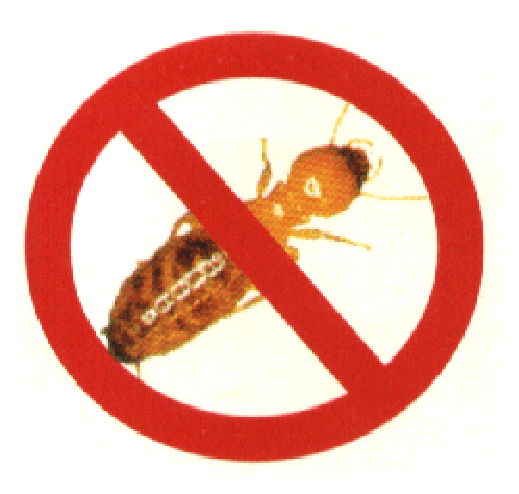
\includegraphics[width=0.5\textwidth]{Cap1/cupim}
    % \caption{Proibido estacionar cupins. Legenda grande, com o objetivo de demonstrar a indentação na lista de figuras.}
    % \label{cupim}
    % \end{figure}

    
    % \begin{figure}[ht!]
    % \centering
    % 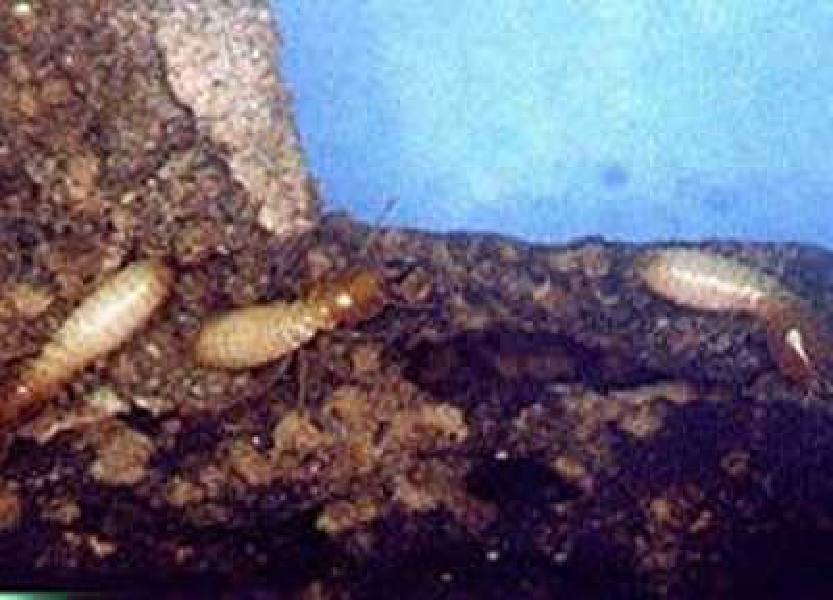
\includegraphics[width=1\textwidth]{Cap1/cupimconcreto}
    % \caption{Exemplo real de cupim frente ao seu dilema.}
    % \label{FDII}
    % \end{figure}
    
    % \begin{figure}[ht]
    % \centering
    % 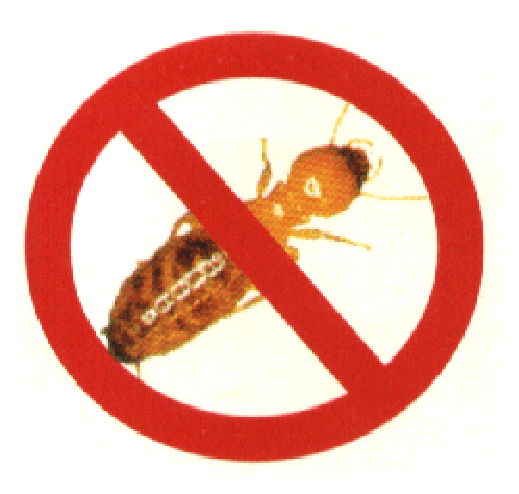
\includegraphics[width=0.5\textwidth]{Cap1/cupim}
    % \caption{Proibido estacionar cupins. Legenda grande, com o objetivo de demonstrar a indentação na lista de figuras.}
    % \label{cupim}
    % \end{figure}
    
    % \begin{figure}[ht!]
    % \centering
    % 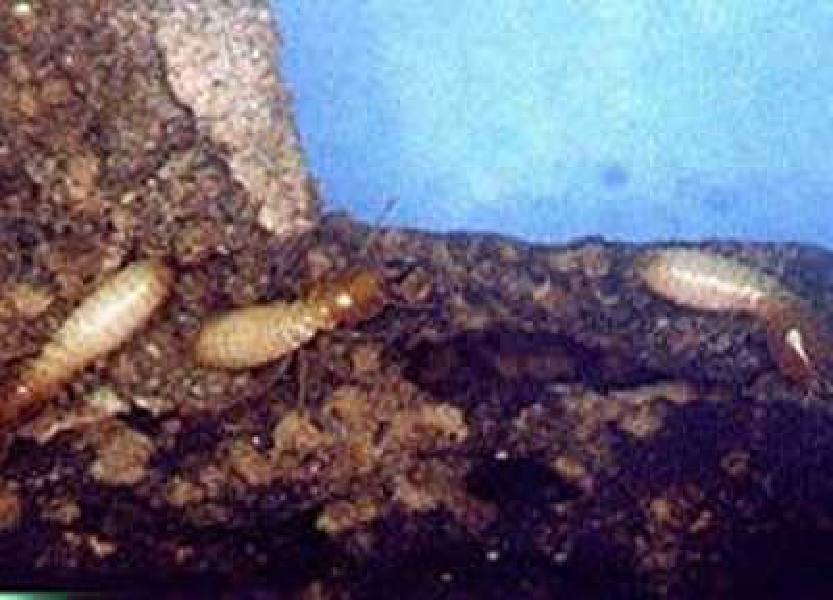
\includegraphics[width=1\textwidth]{Cap1/cupimconcreto}
    % \caption{Exemplo real de cupim frente ao seu dilema.}
    % \label{FDII}
    % \end{figure}
    

\chapter{Método de análise de entropia de composições}
\section{Notação Musical}

Para este trabalho será necessário que um conhecimento prévio de teoria e notação musical moderna. O conhecimento básico necessário para o entendimento do que será exposto a seguir está no Apêndice \ref{ape:notacao}.
Digitalmente, as composições podem ser representadas pelo padrão MIDI.

%%%%%%%%%%%%%%%%%%%%%%%%%%%%%%%%%%%%%%%%%%%%%%%%%%%%%%%%%%%%%%%%%%%%%
\section{Arquivos MIDI}

[ TODO: ]



%%%%%%%%%%%%%%%%%%%%%%%%%%%%%%%%%%%%%%%%%%%%%%%%%%%%%%%%%%%%%%%%%%%%%
\section{Entropia}

[ Falar sobre um pouco sobre processo estocástico ]

Entropia da informação é definida como a quantidade de informação produzida por um processo estocástico. É a grandeza que procura medir a incerteza ou a taxa na qual informação é gerada ou transmitida.

Considerando um evento $X$ que pode assumir os valores ${x_1, x_2, ..., x_n}$, onde se conhece a probabilidade $P(x_i)$ para cada valor, pretende-se medir quanta informação é transmitida por cada valor. Para isso, deve-se encontrar uma função $H(X)$ com as seguintes propriedades \cite{shannon}:

\begin{itemize}
    \item $H$ deve ser contínua em X;
    \item Se $P(x_i)$ é igual para todo $i$, isto é, $P(x_i) = \frac{1}{n}$, então $H$ deve ser monótona crescente em $n$, isto é, para escolhas equiprováveis, quanto mais valores possíveis maior é a incerteza associada;
    \item Se uma escolha pode ser dividida em duas escolhas sucessivas, o valor de $H$ deve ser igual a soma ponderada dos valores individuais de $H$. 
\end{itemize}

A função $H$, entropia de X, que satisfaz as propriedades é \cite{shannon}:

\begin{equation}
    H(X) = - K \sum_{i=1}^{n} P_X(x_i) \log_b{[P_X(x_i)]}
\label{eq:entropy}
\end{equation}
$K$ é uma constante positiva que define a unidade. Será usado o valor $K=1$ aqui em diante. Será utilizado, também, $b=2$. Assim, temos o resultado em bits.

[ TODO: Falar de propriedades ]

%%%%%%%%%%%%%%%%%%%%%%%%%%%%%%%%%%%%%%%%%%%%%%%%%%%%%%%%%%%%%%%%%%%%%
\section{Entropia Condicional}

Pode-se definir Entropia Conjunta de duas variáveis aleatórias $X$ e $Y$ da mesma forma expressa na equação \ref{eq:entropy}, utilizando $(X, Y)$ como uma única variável aleatória vetorial. Já utilizando os valores definidos para $K$ e $b$ temos \cite{livro}:

\begin{equation}
    H(X) = - \sum_{x \in X}\sum_{y \in Y} P(x_i, y_i) \log_2{P(x_i, y_i)}
\label{eq:joint_entropy}
\end{equation}

Esse valor também pode ser representado da seguinte forma \cite{livro}:

\begin{equation}
    H(X) = - E \log_2{P(X, Y)}
\end{equation}

A partir desse valor, pode-se calcular o valor da Entropia Condicional \cite{livro}:

\begin{equation}
    H(Y|X) = - E_{P(X,Y)} \log_2{P(Y|X)}
\end{equation}

A partir do valor da função de probabilidade conjunta $P(X,Y)$, pode-se calcular o valor da Entropia Condicional através da equação \cite{livro}:

\begin{equation}
    H(X) = - \sum_{x \in X}\sum_{y \in Y} P(x_i, y_i) \log_2{\frac{P(x_i, y_i)}{P(x_i)}}
\end{equation}





%%%%%%%%%%%%%%%%%%%%%%%%%%%%%%%%%%%%%%%%%%%%%%%%%%%%%%%%%%%%%%%%%%%%%
\section{Informação Mútua}

É possivel, também, que estude a variável $X$ condicionalmente a outra variável aleatória $Y$. Assim, pode-se calcular a Entropia de $X$ quando se conhece $Y$:

\begin{equation}
    H(X|Y) =  \sum_{j=1}^{m} P_Y(y_i) H(X|Y = y_i)
\end{equation}


%%%%%%%%%%%%%%%%%%%%%%%%%%%%%%%%%%%%%%%%%%%%%%%%%%%%%%%%%%%%%%%%%%%%%
\section{Modelo}

Uma composição musical, ou uma de suas vozes, pode ser observada como uma sequência de notas, acodes e / ou pausas com uma duração associada. Assim, pode-se modelar cada instante da música como duas variáveis aleatórias:

\begin{enumerate}
    \item Nota, Acorde ou Pausa
    \item Duração
\end{enumerate}

Ao realizar o pré-processamento da composição, foram feitas algumas considerações:

\subsection{Extração da Melodia}

Tanto as composições musicais mais clássicas como as mais modernas apresentam diversos instrumentos ou vozes simultaneamente. Dentre as mais clássicas, as mais simples apresentam duas sequências principais:

\begin{itemize}
    \item Base
    \item Melodia
\end{itemize}

No caso de composições mais modernas, há a presença de vários instrumentos musicais, dentre eles:

\begin{itemize}
    \item Voz
    \item Guitarra
    \item Violão
    \item Piano
    \item Contrabaixo
    \item Bateria / Percussão
\end{itemize}

Para propósitos deste trabalho, foi feita a extração apenas da sequência principal, ou melodia, de cada uma das composições utilizadas. Essa extração foi feita utilizando o software MuseScore \cite{musescore}, que permite a vizualização de arquivos MIDI em formato mais amigável para um humano, assim como edição dos mesmos.

% \subsection{Modo}

% Outro fator a se considerar o modo das escalas, que pode ser maior, menor, dentre outros. Nesse trabalho, foram considerados os modos maior e menor apenas. A separação aqui é feita pois há uma diferença entre o significado de uma sequência de notas em uma escala devido ao seu modo, por exemplo, a sequência $C$,$E$, $G$ representa coisas diferntes nas escalas de Dó Maior ou Dó Menor.

\subsection{Altura da nota}\label{section:altura_da_nota}

As notas de mesmo nome observadas em escalas diferentes foram tratadas com o mesmo valor, por exemplo, a nota Dó foi tratada com o mesmo valor se está na primeira oitava ($C_1$) ou na quarta oitava ($C_4$). Isto deve-se ao fato de que, em uma mesma escala, as notas de mesmo nome em oitavas diferentes carregam, muitas vezes, a mesma informação.

\subsection{Acordes}

Para os acordes, foi tomada duas abordagens diferentes:

\begin{enumerate}
    \item Considerar um acorde como um evento próprio, após o devido tratamento que consiste em simplificar as notas em oitavas diferentes, como foi explicitado em \ref{section:altura_da_nota}, e também ignorar a repetição de notas iguais, por exemplo, o acorde ($C3$, $E3$, $C4$) é tratado como ($C$, $E$).

    \item Utilizar a Nota fundamental do acorde para representar o evento. Por exemplo, o acorde ($C3$, $E3$, $C4$), nesse caso, é tratado como a nota $C$ sendo tocada individualmente
\end{enumerate}

As notas de mesmo nome observadas em escalas diferentes foram tratadas com o mesmo valor, por exemplo, a nota Dó foi tratada com o mesmo valor se está na primeira oitava ($C1$) ou na quarta oitava ($C4$). Isto deve-se ao fato de que, em uma mesma escala, as notas de mesmo nome em oitavas diferentes carregam, muitas vezes, a mesma informação.

\subsection{Função probabilidade}

Para as análises de entropia é necessário que estabeleçamos a função de distribuição de probabilidade $P(X)$ dos eventos que serão analisar. Esse valor foi obtido experimentalmente através de análise de frequência das composições que foram estudadas.

\subsection{Distâncias entre notas consecutivas}

Para a análise com a utilização do evento Distância entre notas consecutivas foram tomadas duas abordagens:

\begin{enumerate}
    \item Distância entre as duas notas em semitons, equivalente a diferença do valor MIDI para as duas notas.
    \item Distância entre as duas notas na escala em que a música foi composta.
\end{enumerate}

\subsection{Duração}

A duração dos eventos foi tratada como uma variável aleatória independente do evento. A função de probabilidade também foi obtida através da análise de frequência destes eventos.

%%%%%%%%%%%%%%%%%%%%%%%%%%%%%%%%%%%%%%%%%%%%%%%%%%%%%%%%%%%%%%%%%%%%%
\section{Método de Análise}




\chapter{Análise de composições}
\label{cap:analise}
\section{Tecnologias Utilizadas}

Neste trabalho, foram utilizadas algumas tecnologias e ferramentas que favoreceram e auxiliaram no desenvolvimento.

\subsection{Python 3}

Python é uma linguagem de programação de alto nível, com modelo de desenvolvimento aberto. \cite{python}. Surgiu em 1991 e tem se popularizado pela sua facilidade de aprendizado e simplicidade para implementação de scripts, análises e processamento de dados.

Este trabalho utilizou-se de uma das versões mais recentes da linguagem, que é a versão 3.5.3 (Setembro, 2017). 

\subsection{music21}

Uma biblioteca que contém diversas implementações que auxiliam no estudo da música. \cite{music21}.
Ela foi utilizada para auxiliar na leitura e formatação dos arquivos \textit{MIDI}, assim como o pré-processamento dos dados obtidos destes arquivos.

A biblioteca ainda provê implementação de alguns algoritmos que auxiliam na detecção do tom ou escala em que a composição foi escrita.

\subsection{Jupyter}

Trata-se de um projeto aberto e sem fins lucrativos que auxilia em computações científicas e de processameneto de dados e provê uma interface interativa.


% ===============================================================
\section{Desenvolvimento}

A \textit{framework} desenvolvida é composta por três módulos principais:

\begin{itemize}
    \item \textit{probability.py}: Realiza as análises de frequência de uma composição musical para todos os modelos citados no \ref{cap:metodo}
    \item \textit{entropy.py}: Realiza os cálculos de entropia média e no instante para uma composição.
    \item \textit{graphs.ipynb}: \textit{Jupyter notebook} que gera os gráficos para as análises que serão mostradas a seguir
\end{itemize}

% ===============================================================
\section{Evolução}

O objetivo desta seção é tentar retratar uma evolução da música internacional ao longo dos anos; desde artistas clássicos até os mais modernos. Foram utilizadas 57 composições de um total de 12 artistas e bandas. A composição mais antiga data de 1784 e a mais recente, de 2014. Os artistas utilizados, juntamente com os anos de atividade, são:

\begin{itemize}
    \item Wolfgang Amadeus Mozart (1761 - 1791) \cite{midiworld}
    \item Niccolò Paganini (1793 - 1840) \cite{midimelody}
    \item Frédéric François Chopin (1818 - 1849) \cite{midiworld}
    \item Sergei Vasilievich Rachmaninoff (1877 - 1943) \cite{midiworld}
    \item Scott Joplin (1895 - 1917) \cite{trachtman}
    \item Duke Ellington (1914 - 1974) \cite{midimelody}
    \item Elvis Presley (1953 - 1977) \cite{midiworld}
    \item Antônio Carlos Jobim (1956 - 1994) \cite{wersi}
    \item The Beattles (1960 - 1970) \cite{midiworld}
    \item Pink Floyd (1965 - 1995, 2005, 2012 - 2014) \cite{midiworld}
    \item Dream Theater (1985 - Atualmente) \cite{freemidi}
    \item Taylor Swift (2004 - Atualmente) \cite{freemidi}
\end{itemize}
A figura
% \ref{fig:evo}
mostra o valor médio de entropia de cada composição utilizando como evento o TODO: (nota, cond, dist ou dur). O valor de cada composição está representado com um círculo e o valor médio por artista está representado com um $X$. 

TODO: INSERIR FIGURA

A figura
% \ref{fig:artists}
mostra o valor médio por artista e também apresenta uma escala mais precisa no eixo da entropia.

TODO: INSERIR FIGURA

Nota-se uma pequena difereça entre os compositores mais clássicos (porção mais à esquerda) em relação aos artistas mais modernos, tendo os primeiros valores mais elevados de entropia. Nota-se também que os artistas que 

Para uma comparação mais precisa, as tabelas de
% \ref{tab:mozart} até % \ref{tab:taylor}
mostram os valores de entropia calculados para cada uma das composições em cada um dos modelos já citatos no capítulo \ref{cap:metodo}.
% % Please add the following required packages to your document preamble:
% \usepackage[table,xcdraw]{xcolor}
% If you use beamer only pass "xcolor=table" option, i.e. \documentclass[xcolor=table]{beamer}
\begin{table}[]
\centering
\caption{My caption}
\label{my-label}
\begin{tabular}{|c|c|c|c|c|c|}
\hline
\rowcolor[HTML]{9B9B9B} 
{\color[HTML]{FFFFFF} Composição}                                                                 & {\color[HTML]{FFFFFF} Ano} & {\color[HTML]{FFFFFF} H(Evento)} & {\color[HTML]{FFFFFF} H(Cond)} & {\color[HTML]{FFFFFF} H(Dist)} & {\color[HTML]{FFFFFF} H(Dur)} \\ \hline
\begin{tabular}[c]{@{}c@{}}Piano Sonata\\ No. 11\\ Movement 1\\ Theme and variations\end{tabular} & 1784                       &                                  &                                &                                &                               \\ \hline
\begin{tabular}[c]{@{}c@{}}Piano Sonata\\ No. 11\\ Movement 2\\ Menuetto and trio\end{tabular}    & 1784                       &                                  &                                &                                &                               \\ \hline
\begin{tabular}[c]{@{}c@{}}Piano Sonata\\ No. 11\\ Movement 3\\ Rondo alla turca\end{tabular}     & 1784                       &                                  &                                &                                &                               \\ \hline
Krebsgang                                                                                         & 1785                       &                                  &                                &                                &                               \\ \hline
\begin{tabular}[c]{@{}c@{}}Eine kleine\\ Nachtmusik\end{tabular}                                  & 1787                       &                                  &                                &                                &                               \\ \hline
\end{tabular}
\end{table}

\chapter{Conclusões}
\section{Conclusão}

Neste trabalho, foi apresentado como pode-se medir 

% REFERENCIAS BIBLIOGRAFICAS
\renewcommand\bibname{\itareferencesnamebabel} %renomear título do capítulo referências
\bibliography{Referencias/referencias}

% Apendices
\appendix
\chapter{Notação Musical} %opcional
\section{Notação Musical}\label{ape:notacao}

A matriz de Dilema Linear $M$ e o vetor de torques inerciais $b$,
utilizados na simulação são calculados segundo a formulação 
abaixo:
\begin{equation}
M=\left[ \begin{array}{ccc}
M_{11} & M_{12} & M_{13} \\
M_{21} & M_{22} & M_{23} \\
M_{31} & M_{32} & M_{33}
\end{array} \right]
\end{equation}

\begin{figure}[h]
\centering
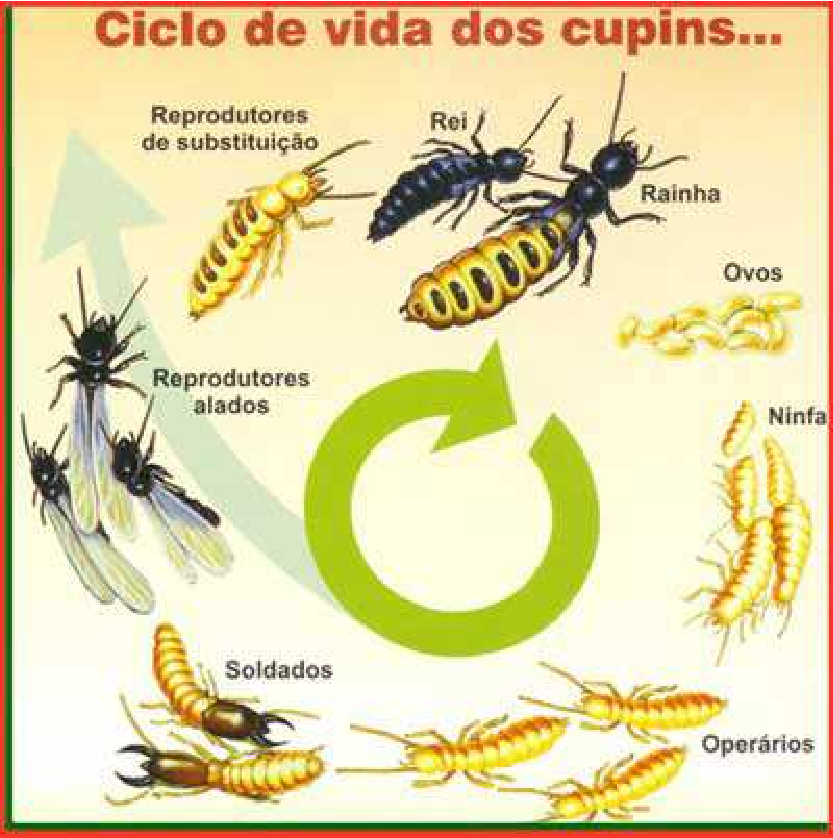
\includegraphics[height=5cm, width=5cm]{ApeA/pragas_ciclo_cupim}
\caption{Uma figura que está no apêndice}\label{FD}
\end{figure}


% Anexos
% \annex
% \chapter{Exemplo de um Primeiro Anexo} %opcional
% % Texto do Primeiro Anexo
\section{Uma Seção do Primeiro Anexo}
% Texto da primeira secao do primeiro anexo
Algum texto na primeira seção do primeiro anexo.



% Glossario
%\itaglossary
%\printglossary

% Folha de Registro do Documento
% Valores dos campos do formulario
\FRDitadata{21 de novembro de 2017}
\FRDitadocnro{DCTA/ITA/TC-117/2017} %(o número de registro você solicita a biblioteca)
\FRDitaorgaointerno{Instituto Tecnológico de Aeronáutica -- Divisão de Engenharia Mecânica -- ITA/IEM}
%Exemplo no caso de pós-graduação: Instituto Tecnol{\'o}gico de Aeron{\'a}utica -- ITA
\FRDitapalavrasautor{Cupim; Cimento; Estruturas}
\FRDitapalavrasresult{Cupim; Dilema; Construção}
%Exemplo no caso de graduação (TG):
%\FRDitapalavraapresentacao{Trabalho de Graduação, ITA, São José dos Campos, 2015. \NumPenultimaPagina\ páginas.}
%Exemplo no caso de pós-graduação (msc, dsc):
\FRDitapalavraapresentacao{ITA, São José dos Campos. Curso de Mestrado. Programa de Pós-Graduação em Engenharia Aeronáutica e Mecânica. Área de Sistemas Aeroespaciais e Mecatrônica. Orientador: Prof.~Dr. Adalberto Santos Dupont. Coorientadora: Prof$^\textnormal{a}$.~Dr$^\textnormal{a}$. Doralice Serra. Defesa em 05/03/2015. Publicada em 25/03/2015.}
\FRDitaresumo{TODO:

Aqui começa o resumo do referido trabalho. Não tenho a menor idéia do que colocar aqui. Sendo assim, vou inventar. Lá vai: Este trabalho apresenta uma metodologia de controle de posição das juntas passivas de um manipulador subatuado de uma maneira subótima. O termo subatuado se refere ao fato de que nem todas as juntas ou graus de liberdade do sistema são equipados com atuadores, o que ocorre na prática devido a falhas ou como resultado de projeto. As juntas passivas de manipuladores desse tipo são indiretamente controladas pelo movimento das juntas ativas usando as características de acoplamento da dinâmica de manipuladores. A utilização de redundância de atuação das juntas ativas permite a minimização de alguns critérios, como consumo de energia, por exemplo.
Apesar da estrutura cinemática de manipuladores subatuados ser idêntica a do totalmente atuado, em geral suas caraterísticas dinâmicas diferem devido a presença de juntas passivas. Assim, apresentamos a modelagem dinâmica de um manipulador subatuado e o conceito de índice de acoplamento. Este índice é utilizado na sequência de controle ótimo do \mbox{manipulador}.
A hipótese de que o número de juntas ativas seja maior que o número de
passivas  $(n_{a} > n_{p})$  permite o controle ótimo das juntas passivas, uma vez que na etapa
de controle destas há mais entradas (torques nos atuadores das juntas ativas), que
elementos a controlar (posição das juntas passivas). }
%  Primeiro Parametro: Nacional ou Internacional -- N/I
%  Segundo parametro: Ostensivo, Reservado, Confidencial ou Secreto -- O/R/C/S
\FRDitaOpcoes{N}{O}
% Cria o formulario
\itaFRD

\end{document}
% Fim do Documento. O massacre acabou!!! :-)
